%ju 16-Mai-22 01-Kostenrechnung.tex
\textbf{Kosten- und Leistungsrechnung} (KLR) $\to$ internes
Rechnungswesen

vs.

\textbf{Buchhaltung} (FiBu) $\to$ externes Rechnungswesen

\textbf{Kosten einteilen}

\begin{itemize}
\item
  Teilkosten: fixe und variable Kosten
\item
  Vollkosten: Einzelkosten und Gemeinkosten
\end{itemize}

\section{Vollkostenrechnung}\label{vollkostenrechnung}

Vgl. Kostenrechnung Fachbuch S. 79-102
(\textcite{heiser:2017:betriebsfuhrung}).

\begin{enumerate}
\item
  \textbf{Einzelkosten} (EK), direkte Kosten (Kunden), Fertigungslöhne
  $\to$ produktive Löhne

  \begin{itemize}
  \item
    \begin{enumerate}
    \def\labelenumii{\alph{enumii}.}
    \setcounter{enumii}{25}
    \item
      B. Fertigungslöhne, Anschaffungskosten, Fertigungsmaterialien
      (Ersatzteile)
    \end{enumerate}
  \item
    $\boxed{\text{FL} = WSL \cdot Flh}$\\
  \item
    (WSL) = (StLs) Werkstattschnittlohn = Stundenlohnsatz
  \end{itemize}
\item
  \textbf{Gemeinkosten} (GK), indirekte Kosten, Hilfslöhne (W-Aufträge)
  $\to$ unproduktive Löhne

  \begin{itemize}
  \item
    \begin{enumerate}
    \def\labelenumii{\alph{enumii}.}
    \setcounter{enumii}{25}
    \item
      B. Reisekosten, Kfz-Aufwendungen, Abschreibungen,
      Zinsaufwendungen, Eigenkapital-Verzinsung (kalkulatorisch)
    \end{enumerate}
  \item
    $\boxed{\text{GK} = Seko - EK} \quad \boxed{\text{GK} = \frac{WSL \cdot GKZs}{100}}$\\
  \end{itemize}
\item
  \textbf{Gemeinkostenzuschlagsatz} (GKZs) in \%

  \begin{itemize}
  \item
    $\boxed{\text{GKZs} = \frac{GK \cdot 100}{FL}}$\\
  \end{itemize}
\item
  \textbf{Kalkulatorische Kosten} Gemeinkosten, die keine Ausgaben
  verursachen; aufwandsfremde Kosten

  \begin{itemize}
  \item
    \begin{enumerate}
    \def\labelenumii{\alph{enumii}.}
    \setcounter{enumii}{25}
    \item
      B. Kalk.-Miete, Kalk.-Abschreibungen, Kalk.-Zinsen, Kalk.-U-Lohn,
      Kalk.-Wagnisse
    \end{enumerate}
  \end{itemize}
\item
  \textbf{Gewinn} (GW) in € Einkommen des Unternehmers, Wagnis,
  Unternehmensrisiko

  \begin{itemize}
  \item
    $\boxed{\text{Gewinn} = UE - EK - GK} \quad \boxed{\text{Gewinn/h} = StVs - Seko/h}$
  \end{itemize}
\item
  \textbf{Gewinnzuschlag} (GWZs) in \%

  \begin{itemize}
  \item
    $\boxed{\text{GWZs} = \frac{GW \cdot 100}{SeKo}}$
  \end{itemize}
\item
  \textbf{Umsatzerlöse, Erlöse} (UE in EUR), Stundenverrechnungssatz
  (StVs in EUR/h)

  \begin{itemize}
  \item
    Betrag für eine Lesitung = Kostendecken + Gewinn
  \item
    $\boxed{UE = EK + GK + GW} \quad \boxed{UE = Seko + GW}$
    (Selbstkosten + Gewinn)
  \item
    $\boxed{StVs = StLs/WSL + GK + GW}$
  \end{itemize}
\item
  \textbf{Selbstkosten} (SeKo)

  \begin{itemize}
  \item
    $\boxed{SeKo = EK + GK}$ (Einzelkosten + Gemeinkosten)
  \item
    $\boxed{SeKo = FL + GK}$ vs.~$\boxed{SeKo/h = WSL + GK/h}$
  \item
    $\boxed{SeKo_{EUR} = UE - GW} \to \boxed{SeKo_\% = 100~\% - UR_\%}$
  \end{itemize}
\end{enumerate}

\begin{figure}[!ht]% hier: !ht
\centering
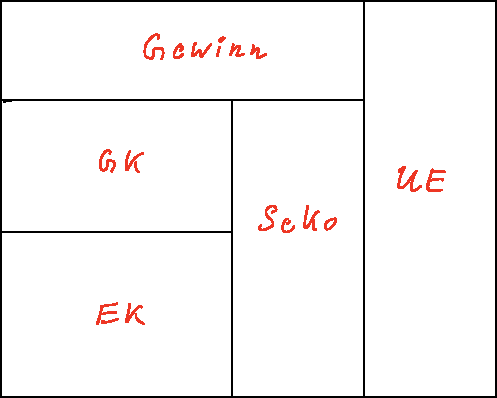
\includegraphics[width=0.4\textwidth]{images/Skizze/02_Umsatzerloese_Skizze.pdf}
\caption{Kosten und Erlöse}
%\label{fig:}%% anpassen
\end{figure}

\newpage

\subsection{Kosten der Werkstatt}\label{kosten-der-werkstatt}

\begin{enumerate}
\item
  \textbf{Fertigungslöhne} (FL), >>produktiv<<, EK, direkt

  \begin{itemize}
  \item
    Auftrag direkt dem Kunden in Rechnung stellen
  \item
    $\boxed{\text{FL} = WSL \cdot Flh}$
  \item
    \begin{enumerate}
    \def\labelenumii{\alph{enumii}.}
    \setcounter{enumii}{25}
    \item
      B. $90~\%$ Lohnkosten
    \end{enumerate}
  \end{itemize}
\end{enumerate}

$+$

\begin{enumerate}
\setcounter{enumi}{1}
\item
  \textbf{Hilfslöhne} (HL) >>unproduktiv<<, GK, nicht direkt, entstehen
  bei Werkstattaufträgen

  \begin{itemize}
  \item
    W-Aufträge z. B. Leerlauf, Nacharbeiten, Reparatur von
    Werkstattfahrzeuge, Urlaub, Feiertage, Wartezeiten
  \item
    \begin{enumerate}
    \def\labelenumii{\alph{enumii}.}
    \setcounter{enumii}{25}
    \item
      B. $10~\%$ Lohnkosten
    \end{enumerate}
  \end{itemize}
\end{enumerate}

$= 100~\%$

\textbf{Fertigungslöhne entstehen bei}

\begin{enumerate}
\item
  \textbf{K-Aufträge}

  \begin{itemize}
  \item
    Kundenauftrag, externe Aufträge
  \item
    \begin{enumerate}
    \def\labelenumii{\alph{enumii}.}
    \setcounter{enumii}{25}
    \item
      B. Wartung, Kundendienst, Reparatur
    \end{enumerate}
  \end{itemize}
\item
  \textbf{I-Aufträge}

  \begin{itemize}
  \item
    interne Aufträge, innerbetrieblich (andere Abteilung des Betriebs)
  \item
    \begin{enumerate}
    \def\labelenumii{\alph{enumii}.}
    \setcounter{enumii}{25}
    \item
      B. Fahrzeugaufbereitung, Gebrauchtwagenreparatur, Überführung,
      Übergabedurchsicht
    \end{enumerate}
  \end{itemize}
\item
  \textbf{G+K-Aufträge}

  \begin{itemize}
  \item
    Garantie- und Kulanzanträge
  \item
    für Kunden ohne Berechnung, Gründe: Kulanz, Sachmängelhaftung,
    Kundenzufriedenheit gewährleisten
  \end{itemize}
\end{enumerate}

\textbf{Zeitlohn vs.~Leistungslohn}

\begin{enumerate}
\item
  \textbf{FL - Zeitlohn} Fertigungslohn, produktive Arbeitszeit,
  Stundenlohn

  \begin{itemize}
  \item
    \textbf{FLh} Fertigungslohnstunden
  \item
    \textbf{WSL} Werkstattschnittlohn, quer durch die Werkstatt z. B.
    Lehrling, Geselle

    \begin{itemize}
    \item
      $\boxed{\text{WSL} = \frac{FL}{Flh}}$
    \end{itemize}
  \item
    \textbf{MAZ} Mehrarbeitszuschlag
  \end{itemize}
\item
  \textbf{FL - Leistungslohn} Lohn für die erbrachte Leistung

  \begin{itemize}
  \item
    \textbf{AWLs} Arbeitswertlohnsatz
  \item
    \textbf{ZELs} Zeiteinheitenlohnsatz
  \item
    \textbf{Soll-AW} Vorgabe, wie viele AW muss ich in einer Stunde
    machen?
  \item
    \textbf{Ist-AW} tatsächlich erbrachte Leistung
  \item
    \textbf{Mehr-AW} Mehrleistung in AW
    $\boxed{\text{AW} = \text{Ist-AW} - \text{Soll-AW}}$
  \end{itemize}
\end{enumerate}

\textbf{Vorgabezeiten} Grundlage für Leistungslohn

\begin{itemize}
\item
  \textbf{ZE} Zeiteinheit (in Min.)

  \begin{itemize}
  \item
    (StVs / 60 = €/ZE x Min. = Preis (€))
  \end{itemize}
\item
  \textbf{AW} Arbeitswert (in Min.) Richtzeiten, Vorgabezeiten
\item
  \textbf{WF} Werkstattfaktor $\to$ wie viele AW/ZE in einer Stunde?
  (Soll-Leistung, Mindestleistung)

  \begin{itemize}
  \item
    (12 AW/h = $\frac{60}{12}$ alle 5 Min. 1 AW)
  \end{itemize}
\item
  \textbf{LF} Leistungsfaktor (Ist-Leistung)
\end{itemize}

\newpage

\subsection{Kennwerte der Werkstatt}\label{kennwerte-der-werkstatt}

\begin{enumerate}
\item
  \textbf{Soll-Umsatzerlös} (Soll-UE) deckt die Selbstkosten ab

  \begin{itemize}
  \item
    Soll-UE = Seko + GW
  \end{itemize}
\item
  \textbf{Ist-Umsatzerlös} tatsächlich erwirtschaftete Umsatz
\item
  \textbf{Lohnerlöse} Umsatzerlöse
\item
  \textbf{Wirtschaftlichkeit} (WI) wurde Gewinn oder Verlust gemacht z.
  B. 1,05 \% $\to$ 5 \% mehr

  \begin{itemize}
  \item
    Wirtschaftlichkeit = Umsatzerlöse / Selbstkosten
  \item
    WI = LE / Seko; WI = UE/Seko
  \item
    WI > 1 Gewinn
  \item
    WI \textless{} 1 Verlust
  \item
    WI = 1 Kostendeckend
  \end{itemize}
\item
  \textbf{Produktivität} (PR)

  \begin{itemize}
  \item
    Gesamte Arbeitszeit (Fertigungs- + Hilfslohnstunden)
  \item
    Produktivität = Fertigungslohnstunden x 100 / Arbeitszeit
  \item
    PR = FLh x 100 / AZ\\
  \end{itemize}
\item
  \textbf{Leistungsfaktor} (LF)

  \begin{itemize}
  \item
    tatsächlich erbrachte Leistung je Stunde
  \item
    Leistungsfaktor = Ist-Leistung in AW / Fertigungslohnstunden
  \item
    LF = Ist-AW / FLh
  \end{itemize}
\item
  \textbf{Leistungsgrad} (LG)

  \begin{itemize}
  \item
    $\boxed{\text{LG} = \frac{\text{Ist-AW}}{\text{Soll-AW}}}$
  \item
    (Ist-Leistung / Soll-Leistung) und (tatsächlich erbrachte Leistung /
    Mindestleistung)
  \end{itemize}
\item
  \textbf{Leistungslohnsatz}

  \begin{itemize}
  \item
    Leistungslohnsatz = Fertigungslohn / Fertigungslohnstunden
  \item
    LLs = FL / FLh
  \end{itemize}
\item
  \textbf{Umsatzrentabilität} (UR) in \%
\end{enumerate}

\begin{itemize}
\item
  Wie viel Prozent des Umsatzes als Gewinn anfallen
\item
  $\boxed{\text{UR} = \frac{GW \cdot 100}{UE}} \quad \boxed{\text{UR} = \frac{GW/h \cdot 100}{StVs}}$
\end{itemize}

\subsubsection{Kostenindex - Stundenverrechnungssatz - AW-Vs
(Prüfung)}\label{kostenindex-stundenverrechnungssatz-aw-vs-pruefung}

\emph{3x wichtige Formeln}

\textbf{Kostenindex, Werkstattindex, Faktor} (KI) wievielmal mehr der
Kunde für eine Fertigungslohnstunde zu bezahlen hat, als der Monteur in
dieser Stunde verdient. (bezieht sich auf Löhne)

$\boxed{\text{KI} = \frac{\text{Prod. Löhne} + \text{GK} + \text{Gewinn}}{\text{Prod. Löhne}}} \quad$
$\boxed{\text{KI} = \frac{\text{StVs}}{\text{WSL}}} \quad \boxed{\text{KI} = \frac{\text{UE}}{\text{FL}}}$

\textbf{Stundenverrechnungssatz} Arbeitspreis, der dem Kunden für eine
Stunde berechnet wird. Reparaturstunde = Fertigungslohnstunde

$\boxed{\text{StVs} = \frac{\text{UE}}{\text{FLh}}} \quad \boxed{\text{StVs} = \text{KI} \cdot \text{WSL}}$

$\boxed{\text{StVs}_{neu} = \frac{\text{Seko}_{neu} \cdot 100~\%}{\text{Seko}_{alt}}} \quad \boxed{\Delta \text{StVs} = \text{StVs}_{neu} - \text{StVs}_{alt}}$

Erhöhung
$\boxed{\text{StVs}_\% = \frac{\Delta \text{StVs} \cdot 100~\%}{\text{StVs}_{alt}}}$

\textbf{AW-Verrechnungssatz} Ermittlung des Arbeitspreises für eine
Arbeitsposition (Leistungslohn)

Erlös je AW

$\boxed{\text{AW-Vs} = \frac{\text{StVs}}{\text{WF}}} \quad \boxed{\text{AW-Vs} = \frac{\text{WSL} \cdot \text{KI}}{\text{WF}}} \quad \boxed{\text{AW-Vs} = \frac{\text{UE}}{\text{FLh} \cdot \text{WF}}}$

\subsubsection{Reparaturkosten
berechnen}\label{reparaturkosten-berechnen}

\textbf{Rechnungserstellung - Formvorschriften beachten}

\begin{itemize}
\item
  Rechnung schriftlich mit Rechnungsnummer und Leistungsdatum
\item
  Kunden- und Fahrzeugdaten wichtige aufführen
\item
  Arbeitskreis und Ersatzteilpreise detailliert aufführen
\item
  Netto-Rechnungsbetrag, Umsatzsteuer, Altteilesteuer und
  Brutto-Rechnungsbetrag einzeln aufführen.
\end{itemize}

\lstset{language=Bash}% C, TeX, Bash, Python 
\begin{lstlisting}[
	%caption={}, label={code:}%% anpassen
]
  Arbeitspreis      = Flh x StVs
+ Materialkosten  
= Reparaturkosten 
+ Umsatzsteuer        19 % 
_____________________________________________
= Rechnungsbetrag                         EUR
\end{lstlisting}

\newpage

\subsection{Handelswarenkalkulation}\label{handelswarenkalkulation}

\textbf{Kalkulationsarten} Vorwärts-, Rückwärts-, Differenzkalkulation

\subsubsection{Einkaufskalkulation}\label{einkaufskalkulation}

\lstset{language=Bash}% C, TeX, Bash, Python 
\begin{lstlisting}[
	%caption={}, label={code:}%% anpassen
]
  BP                                           LEP                 // 100 %
- BK                                         - Rabatt       10 %                 
= BEP                           // 98 %      = ZEP                 // 100 % 
+ Skonto    2 % (in 100)                     - Skonto        2 %
= ZEP                           // 90 %      = BEP                 
+ Rabatt   10 % (in 100)                     + BK
________________________________             ______________________         
= LEP                           EUR          = BP                  EUR 
\end{lstlisting}

\begin{enumerate}
\item
  \textbf{Listeneinkaufspreis} (LEP), Ware, Angebot,
  $\boxed{BEP + \text{Skonto} + \text{Rabatt}}$
\item
  \textbf{Lieferantenrabatt} (LRa), Preisnachlass
\item
  \textbf{Zieleinkaufspreis} (ZEP), Zahlungszeitpunkt, Kauf auf Ziel
  $\boxed{BEP + \text{Skonto}}$
\item
  \textbf{Lieferantenskonto} (LSk)
\item
  \textbf{Bareinkaufspreis} (BEP), bei sofortiger Barzahlung
\item
  \textbf{Bezugskosten} (BK), Transport: Verpackung, Fracht, Zoll,
  Rollgeld
\end{enumerate}

\subsubsection{Verkaufskalkulation,
Ersatzteilkalkulation}\label{verkaufskalkulation-ersatzteilkalkulation}

\lstset{language=Bash}% C, TeX, Bash, Python 
\begin{lstlisting}[
	%caption={}, label={code:}%% anpassen
]
  BP                                           LVP                 // 100 %
+ GK       20 % (auf 100)                    - Rabatt       10 %                 
= SEKO                                       = ZVP                 // 100 %
+ Gewinn    8 % (auf 100)                    - Skonto        2 %
= BVP                           // 98 %      = BVP        
+ Skonto    2 % (in 100)                     - Gewinn
= ZVP                           // 90 %      = Seko                 
+ Rabatt   10 % (in 100)                     - GKZs
________________________________             ______________________          
= LVP                           EUR          = BP                  EUR
+ UST      19 %                                                 
________________________________                        
= Rechnungsbetrag ohne Rabatt   EUR                                 
\end{lstlisting}

\begin{enumerate}
\item
  \textbf{Bezugspreis} (BP), Anschaffungskosten, Einstandspreis
  $\boxed{BEP + BK}$
\item
  \textbf{Gemeinkosten} (GK), anteilig, nicht direkt
\item
  \textbf{Selbstkosten} (SEKO), Beschaffung, Bereitstellung,
  Weiterverarbeitung
\item
  \textbf{Gewinn} Wagnis, U-Lohn
\item
  \textbf{Verkaufssonderkosten} Garantie, Provision, Kundendienst
\item
  \textbf{Barverkaufspreis} (BVP) $\boxed{BP + GK + \text{Gewinn}}$
\item
  \textbf{Kundenskonto} (KSk)
\item
  \textbf{Zielverkaufspreis} (ZVP)
  $\boxed{BP + GK + \text{Gewinn} + \text{Skonto}}$
\item
  \textbf{Kundenrabatt} (KRa)
\item
  \textbf{Listenverkaufspreis} (LVP)
  $\boxed{BP + GK + \text{Gewinn} + \text{Skonto} + \text{Rabatt}}$
\end{enumerate}

\subsubsection{Kalkulationsfaktor}\label{kalkulationsfaktor}

Vgl. Tabellenbuch S. 61 und 69 (\textcite{bell:2021:tabellenbuchKfz}).

\begin{figure}[!ht]% hier: !ht
\centering
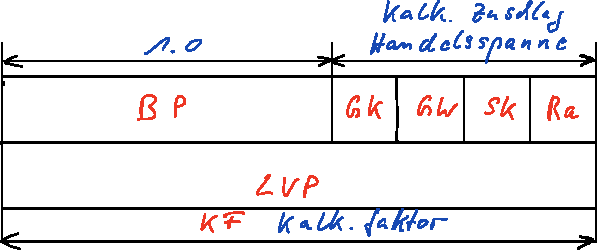
\includegraphics[width=0.6\textwidth]{images/Skizze/03_Kalkulationsfaktor_Skizze.pdf}
\caption{Kalkulationsfaktor}
%\label{fig:}%% anpassen
\end{figure}

\textbf{Kalkulationsfaktor} (KF) wievielmal höher der (Verkaufspreis =
Listenpreis) gegenüber (Bezugspreis) bezieht sich auf das Lager,
Ersatzteil

$\boxed{KF = \frac{LVP}{BP}} \quad \to \boxed{LVP = BP \cdot KF}$

\textbf{Kalkulationszuschlag} enthält
$(GK + \text{Gewinn} + \text{Skonto} + \text{Rabatt})$ bezogen auf
(Bezugspreis)

\textbf{Handelsspanne} (HSP) unterschied zwischen (Verkaufspreis +
Bezugspreis) bezogen auf (Verkaufspreis)
$\boxed{HSP_\% = \frac{HSP \cdot 100}{LVP}}$
$\boxed{HSP_\text{EUR} = LVP - BP}$

\subsubsection{Verkauf von Tauschteilen und
Agenturwarenverkauf}\label{verkauf-von-tauschteilen-und-agenturwarenverkauf}

\textbf{Altteilesteuer} (AT-St) kauft ein Kunde ein Tauschteil und gibt
dabei sein defektes Teil (Altteil) in Zahlung, fällt Altteilesteuer an.
$\boxed{LVP \cdot 10~\% \cdot 19~\%}$

\textbf{Agenturwaren} sind Waren, die im Auftrag und auf Rechnung einer
Fremdfirma verkauft werden (Preise inkl. Gesetzl. Ust.).
